\documentclass[12pt,letterpaper,twoside]{article}
\usepackage[utf8]{inputenc}
\usepackage[spanish]{babel}
\usepackage{setspace}
\spacing{1.5}
\usepackage{amsmath}
\usepackage{amsfonts}
\usepackage{amssymb}
\usepackage{makeidx}
\usepackage{graphicx}
\usepackage{lmodern}
\usepackage{kpfonts}
\usepackage{fourier}
\usepackage[left=2cm,right=2cm,top=2cm,bottom=2cm]{geometry}
\author{Williams Aranguiz}
\title{Proyecto semestral}
\usepackage {fancyhdr}
\usepackage{float}
\usepackage{hyperref}
\hypersetup{
    colorlinks,
    citecolor=black,
    filecolor=black,
    linkcolor=black,
    urlcolor=black
}
\begin{document}

\begin{titlepage}
\centering
{\vspace{1cm}
{\bfseries\LARGE Instituto profesional Duoc UC \par}
\vspace{0.7cm}
{\scshape\Large ESCUELA DE
INFORMÁTICA Y TELECOMUNICACIONES\\
INGENIERÍA INFORMÁTICA.\par}
\vspace{1.5cm}

\includegraphics[width=0.5\textwidth]{Figuras/Logo-AIA.jpeg}\par}

{\scshape\LARGE Sistema de votaciones \par}
{\scshape\large Proyecto semestral \par}
\vspace{3cm}
{\normalsize Autores: Williams Aránguiz A- Angélica Moreno Diaz.\par
}

\vspace{0.5cm}
\raggedleft
{\itshape\normalsize Profesor: Víctor Hugo Rojas Concha\par}
{\itshape\normalsize Diseño de prototipos \par}
%\vfill

\centering
\vfill
{\Large 2021 \par}
\end{titlepage}
\thispagestyle{empty}
\newpage

\newpage
\tableofcontents
\thispagestyle{empty}

\setcounter{page}{1}
\pagestyle{fancy}
\fancyhead{} % clear all fields 
\fancyhead[RO,LE]{
 Proyecto semestral} 
\fancyhead[LO,RE]{AIA}
\fancyfoot{}
\fancyfoot[LE,RO]{Sistema de votaciones} 
\fancyfoot[LO,RE]{\thepage} 
\renewcommand{\headrulewidth}{0.4pt} 
\renewcommand{\footrulewidth}{0.4pt} 

\section{Consultora}
\subsection{Quienes somos}

\begin{figure}[h!]
\centering

\includegraphics[width=7cm]{Figuras/Logo-AIA.jpeg}
\end{figure}

\textbf{AIA} Es la empresa numero 1º en el mercado en soluciones tecnológicas,  dando versatilidad a sus proyecto y velando por las necesidades de sus clientes.

\subsection{Misión}
Buscar la excelencia y simplicidad en los proyectos,  innovando continuamente en áreas de interés mundial,   \textbf{AIA} es un precursor de talento,  por lo cual educar,  formar y actualizar a profesionales colaboradores es el pilar fundamental  dentro de la compañía fomentado a crear un mundo mejor.

\subsection{Visión}
\textbf{AIA} posee como visión mejorar en mundo en sus distintos áreas,  por lo cual,  ser la empresa principal en Chile en la generación de patentes y dominar el mercado TI al 2025 a nivel latinoamericano, tanto en soluciones de \textit{software} y \textit{hardware} integrado. 

"\textbf{\textit{Silicon valley}} es el pasado, el presente le pertenece a las \textbf{\textit{sillicon towns}},  pero el futuro es \textbf{AIA}"




\section{Equipo}
\subsection{Williams Aránguiz - Product owner}
\begin{figure}[h!]
\centering

\includegraphics[width=7cm]{Figuras/Williams.png}
\end{figure}

En concreto, el \textit{Product Owner} procura que el equipo \textit{Scrum} aporte valor al negocio en cuestión. Él representa a los \textit{stakeholders} o a las partes interesadas.

Se encarga de obtener el máximo valor posible al mínimo costo. También es el responsable de la cartera de productos, conocida como pila de producto o \textit{Product Backlog}.  Por esta razón,  comprende las necesidades de los usuarios dentro del negocio.

En la ejecución de los proyectos ágiles, el \textit{Product Owner} normalmente posee las siguientes responsabilidades:

\begin{itemize}
\item Determinar los requisitos generales y actividades iniciales del proyecto.
\item Representar a los usuarios del producto.
\item Buscar y asegurar los recursos financieros que requiere el proyecto para iniciarse y desarrollarse.
\item Analizar la viabilidad del emprendimiento.
\item Garantizar que el producto se entregue.
\item Desarrollar y establecer los criterios para aceptar las historias de los usuarios.
\item Aprobar o negar los productos entregables.
\end{itemize}





\section{Problemática}

\subsection{Caso de estudio}
\begin{figure}[h!]
\centering

\includegraphics[width=7cm]{Figuras/caso.jpg}
\caption{Votaciones para estudiantes}
\end{figure}

En nuestras sedes existe un proceso democrático asociado a la elección de consejeros de carrera,
estos alumnos son elegidos por votación una vez al año, muchas veces en las diferentes sedes
ocurren situación especiales en las cuales los consejeros deben hacer llegar inquietudes a los
directores de carreras o de sede, o recibir de parte de ellos alguna propuesta las cuales deben
transparentar con sus compañeros, en ambas situaciones, sería de mucha ayuda para los
consejeros saber lo que realmente piensan sus compañeros.

En las sedes no existe infraestructura o algún servicio que pueda ayudar a los consejeros con esta
compleja situación, además, cada vez es más necesario contar con la opinión real del estudiantado.

Se requiere que se proponga un conjunto de opciones e ideas que puedan entregar una solución a
está problemática. 


\section{Estado del arte}

\subsection{Aplicaciones de voto electrónico}
Según la pagina web http://www.dit.upm.es:

Lo primero que hay que hacer constar es que no existe en la actualidad ningún software, tanto libre como propietario, que cumpla con todos los requerimientos explicitados en este ensayo para ser considerado como un sistema completo de voto electrónico. Podemos clasificar los sistemas existentes en diversas categorías:

\subsubsection{Sistemas de toma de decisiones}
Existen multitud de soluciones propietarias para el problema de la toma de decisiones. En general, estas soluciones, son módulos adicionales a programas de videoconferencia, trabajo cooperativo, etc.

\subsubsection{Sistemas de recuento de votos}
Del mismo modo existen sistemas electrónicos para el proceso de conteo de resultados. Detallaremos por su "fama" dos de ellos:

\begin{itemize}
\item En algunos estados de USA, el voto no se efectua en una urna, sino a través de un mecanismo similar a una máquina tragaperras: El votante, una vez autentificado y autorizado su voto, accede a una cabina, en la que en dicha máquina selecciona el voto deseado, y lo emite. El recuento es automático, y al finalizar la jornada electoral se obtienen directamente los resultados.
\item Una empresa española ha creado un sistema de recuento automático basado en el reconocimiento del voto a través de un lector óptico. El votante inserta el voto a la manera habitual en la urna, disponiendo ésta de un lector óptico que reconoce un código de barras incorporado en la papeleta. Este sistema es actualmente propiedad del Gobierno Vasco, y está pendiente de autorización gubernamental.

\end{itemize}

\subsubsection{Sistemas de encuestas y consultas anónimas}
Es muy corriente en el Software Libre la existencia de programas de consulta. Portales, como Slashdot, BarraPunto, Technocrat, etc son foros de discusión donde se proponen diversos temas de actualidad, noticias, etc. Incluyen además sistemas de encuestas, donde los participantes en los foros manifiestan su opinion sobre un tema propuesto por los editores.

\subsubsection{Sistemas de voto}
Una nueva categoría constituyen los programas de voto propiamente dicho

El primer caso son aquellos sistemas simples, sin posibilidad de reconfiguración: un ejemplo lo tenemos en MyPools desarrollado por Josh Levine (josh@levinenet.com), basado en PHP y MySQL. En este programa, el administrador edita un fichero de configuración, donde se define la consulta y las opciones. Mediante cookies, se guardan las votaciones y sus resultados.

En general este y otros programas similares están orientados a una única votación sobre un tema concreto. El administrador es quien define los datos de la encuesta, teniendo que proceder manualmente a la mayor parte de las operaciones. El usuario no tiene ningún sistema de realimentación para recepción de claves.

\subsubsection*{Servidor de voto comercial: E-Vote}

Una empresa alemana E-Vote ofrece diversos servicios de toma de decisiones distribuída.  Para ello alquila una aplicación que actúa como cliente de sistemas Windows, y que permite conectarse a un servidor de toma de decisiones.

\begin{figure}[h!]

\centering
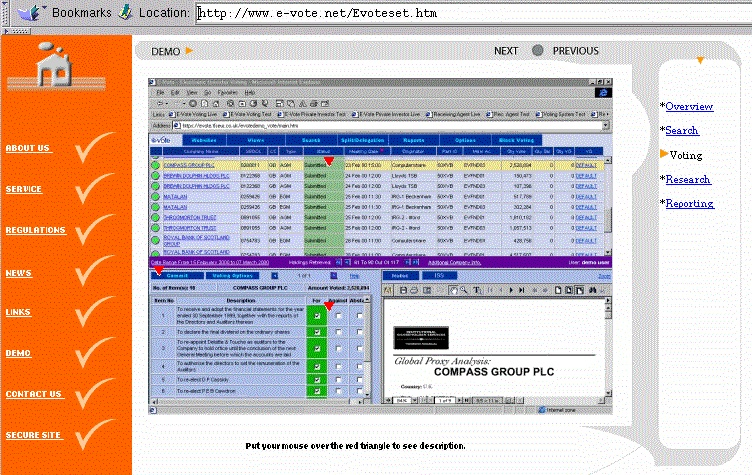
\includegraphics[width=10cm]{Figuras/evotenet.jpg}
\caption{E-Vote Servidor comercial de consultas electrónicas }
Autor: http://www.dit.upm.es
\end{figure}

Dicha aplicación tiene todas las características que se esperan de un sistema de voto:

\begin{itemize}
\item Sistema de registro de usuarios
\item Elaboración de consultas y votaciones
\item Foro de discusiones
\item Mecanismos de chat y videoconferencia en línea
\item Planificadores de actividades
\end{itemize}

La empresa alquila el servidor a las diversas organizaciones que quieren utilizar sus herramientas de decisión. El servidor en sí mismo no se vende: solo la aplicación cliente

Se utilizan mecanismos especiales para identificar unívocamente a los usuarios, y garantizar la unicidad y secreto del voto, así como para cumplir la reglamentación europea sobre tratamiento de datos personales.

Realmente, más que un sistema de voto es un sistema de toma de decisiones, orientado a entornos de telereunión y teletrabajo.

\subsubsection*{Ejemplo de sistema de voto: \textbf{\textit{Free-Vote}}}

En vista de la carencia en el mundo del software libre de este tipo de programas, el autor ha desarrollado uno que, sin tener una validez plena a efectos legales, cubre la mayor parte de los requisitos de los sistemas de voto electrónico. se trata de \textbf{\textit{Free-Vote}}.

\begin{figure}[H]
\centering
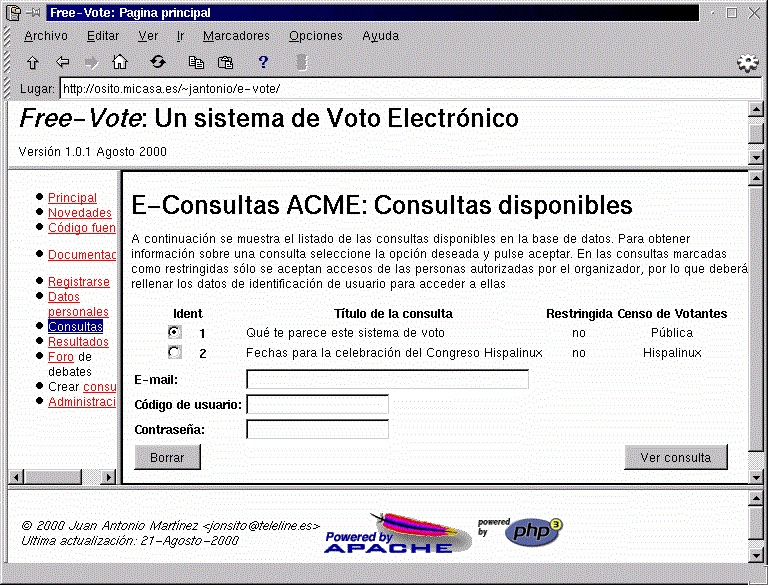
\includegraphics[width=10cm]{Figuras/free-vote.jpg}
\caption{Free-Vote, un programa GPL de voto electrónico }
Autor:  http://drake.dit.upm.es/~jantonio/e-vote/evote.tgz.
\end{figure}

\textbf{\textit{Free-Vote}} ha sido diseñado para servir y dar soporte a sistemas de votación electrónica con un nivel razonable de seguridad y fiabilidad. Las características principales de \textbf{\textit{Free-Vote}} son:

\subsubsection*{Multiconsulta}
Se pueden realizar y monitorizar simultáneamente varias consultas.

\subsubsection*{Configurable}
Cada consulta tiene diversos parámetros, definibles por el organizador de la consulta:

\begin{itemize}
\item Consulta pública o restringida
\item Datos de consulta públicos o privados
\item Foros de debate sobre las diversas consultas
\item Periodos de notificación, registro, y votación
\item Control de información disponible durante la consulta:
	\begin{itemize}
	\item Acceso a listas de votantes
	\item Saber si un votante ha votado o no
	\item Datos sobre porcentajes de participacion
	\item Datos sobre resultados parciales de la consulta
	\end{itemize}
\item Selección y definición de las opciones de voto

\end{itemize}

\subsubsection*{Autentificación de votantes}
Cada votante recibe al realizar la acreditación una tarjeta de voto, válida una única vez.

\subsubsection*{Garantía de voto único y secreto}
El sistema sólo registra si el usuario ha votado o no, nunca el valor de su voto.

\subsubsection*{Control de acceso}
En consultas privadas sólo tienen derecho a voto aquellos votantes definidos por el organizador.

\subsubsection*{Administración distribuída}
El papel del administrador, aunque importante, es secundario: existen diversas categorías de usuarios, cada uno con un nivel de privilegios definible, que permiten una administración distribuída del sistema: alta y baja de usuarios, de consultas, acceso al sistema, etc. Además, punto funtamental en cuanto a seguridad: no hacen falta privilegios de root para su instalación y ejecución.

\subsubsection*{Documentación y procedimientos de instalación automatizados}
Se proporciona una documentación completa en formato SGML, así como diversos scripts de instalación y configuración. Dicha documentación y scripts, han sido escritos de manera que sean conformes a los reglamentos de aplicación de la LORTAD.

El usuario empieza por registrarse en el sistema, obteniendo una clave de acceso. Posteriormente, puede seleccionar las diversas consultas disponibles, y en función de su autorización o no puede emitir voto en aquellas en las que esté autorizado. Para ello debe solicitar una tarjeta de voto, que añade a sus datos de registro una clave adicional para proceder al voto en una votación concreta. La tarjeta de voto es única por cada usuario y cada consulta

Si su nivel de privilegio lo permite, un usuario puede crear y definir consultas, e insertarlas en el sistema. En función del privilegio asignado podrá dar de alta usuarios, autorizar consultas, etc. El máximo nivel de privilegio otorga acceso vía Web a la consola SQL de la base de datos, lo que permite actuar de Administrador

Free-Vote Está basado en PHP-3.0 y PostgreSQL-7.0. Para la elaboración de las páginas web se utiliza en aras de la compatibilidad HTML-3.0 sin extensiones adicionales. Una copia de la última versión del código fuente está disponible vía web en http://drake.dit.upm.es/~jantonio/e-vote/evote.tgz. Se distribuye bajo Licencia GPL.


\subsubsection*{Sistemas de voto basados en correo electrónico:}
El mundo del Software Libre ofrece muchas más posibilidades que el web a la hora de poder realizar aplicaciones de voto electrónico. Vamos a estudiar ahora un sistema de voto basado en el uso del correo: Vote-Debian.

\begin{figure}[H]
\centering
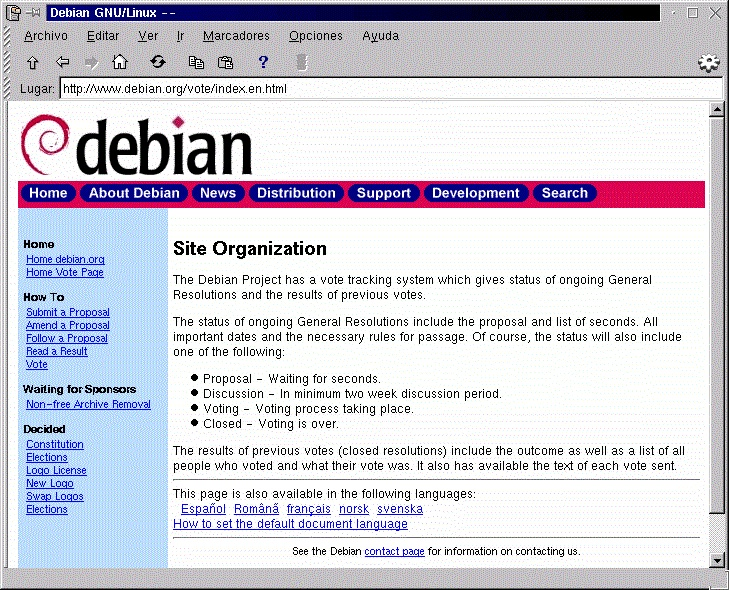
\includegraphics[width=10cm]{Figuras/debian.jpg}
\caption{Vote-Debian, Sistema de voto basado en correo electónico}
Autor:  http://vote.debian.org
\end{figure}

Vote Debian es un sistema enteramente basado en el correo electónico, y enteramente integrado en la filosofía de desarrollo de debian. El proceso de toma de decisión consta de las siguientes fases:

\begin{itemize}
\item \textbf{Propuesta }en la que se manda un mensaje a debian-vote@debian.org en la que se especifican los puntos de discusión, las motivaciones y los textos de la consulta
\item \textbf{Debate} Fase en la que los participantes discuten a través del correo la propuesta, añadiendo enmiendas, o modificando los contenidos
\item \textbf{Votación} Donde se procede al voto. Existen unos formularios predeterminados para la elaboración y tratamiento automatizado del voto
\item \textbf{Resultados} En los que los participantes reciben los resultados de las votaciones, y se adoptan las decisiones pertinentes.

\end{itemize}

Debian Vote es un sistema de toma de decisiones orientado a decidir el funcionamiento interno del grupo de desarrolladores de Debian. Desde este punto de vista es completamente funcional, si bien, desde los aspectos tratados en este artículo tiene estas particularidades:

\begin{itemize}
\item No se garantiza el secreto del voto. De hecho el contenido y resultado de las votaciones es público
\item La autentificación del votante se realiza vía PGP. Existe un registro previo de usuarios

\end{itemize}

Las páginas web de Debian Vote se encuentran en http://vote.debian.org


\subsubsection*{Sistemas de voto basados en IRC}
En general, podemos observar que cualquier sistema electónico que sirva para la comunicación multipunto puede ser empleado para realizar tareas de toma de decisión. Vamos a describir someramente un posible ejemplo de realización a través del Internet Relay Chat (IRC o Chat)

La idea básica del voto a través de IRC consiste en la existencia de un bot, un usuario automático que supervisa todas las actividades relacionadas con el proceso de votación. Los bots son ampliamente utilizados en los sistemas de IRC para muchas aplicaciones. El voto electrónico no es es sino otra aplicación más

La organización es como sigue:

\begin{itemize}

\item Existe un canal de información \#vote\_info donde se anuncian las diversas votaciones en curso
\item Existe un canal \#vote\_xxxx por cada consulta,  que actua como foro de debates
\item Existe un bot que realiza las siguientes operaciones
	\begin{itemize}
	\item Presentación de resultados
	\item Recogida de votos
	\item Control de accesos
	\item Registro de usuarios
	\end{itemize}
\item Por lo general, este bot está asociado a una base de datos, al estilo de un sistema vía web
\item Para proceder a una votación el usuario debe registrarse en el canal asociado, y proceder al voto
\end{itemize}

\begin{figure}[h!]
\centering
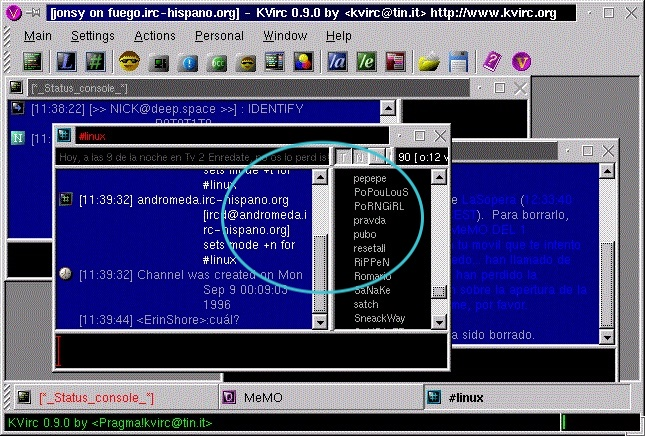
\includegraphics[width=10cm]{Figuras/kvirc.jpg}
\caption{KvIRC, un programa de chat}
Autor:  Internet Relay
\end{figure}

El principal problema de este sistema es el de la autentificación del usuario: IRC está basado en aliases y "nicks", de manera que son necesarios mecanismos adicionales de identificación.

\subsubsection{Otros sistemas de voto electrónico. Consideraciones}
Como hemos comentado el mundo del voto electónico no acaba aquí cualquier sistema que permita comunicación multipunto podría ser utilizado para consultas y votaciones. Citemos algunos ejemplos:

\begin{itemize}
\item Servidores de noticias
\item Sistema de mensajería de los teléfonos móviles
\item Servicios de televisión vía satélite y por cable
\end{itemize}

En general cualquier sistema que tenga una estructura cliente-servidor puede servir. No estamos restringidos en absoluto a los sistemas basados en equipos informáticos. No obstante hay que tener en cuenta una serie de consideraciones:

\begin{itemize}
\item deben garantizarse las premisas que definen el voto:
	\begin{itemize}
	\item Unicidad
	\item Secreto
	\item Autentificación del votante
	\item Libertad de acceso y de voto
	\end{itemize}
\end{itemize}

Con la tecnología actual el principal problema reside en la autentificación del votante. Un ejemplo sencillo: en un sistema de voto basado en mensajes de móviles, no hay garantia de que quien envíe el mensaje sea el propietario del teléfono...

No obstante, y debido a la necesidad que en éste y otros aspectos existe sobre el tema identificación, se están desarrollando diversas técnicas de autentificación: reconocimiento de voz, identificación de huellas, etc. Si bien el principal objetivo es el econónico ( piénsese en la telecompra por teléfono móvil ) el ámbito de actuación de estas técnicas incluye -por supuesto- el voto.

Otro problema asociado a la tecnología es el de la universalidad: Cualquiera que sea el sistema de voto escogido, se debe poder garantizar el que todo aquel que esté interesado tenga posibilidades de participar. Es preciso un acceso universal a las tecnologías asociadas a la toma de decisiones. No puede tolerarse el que existan "no-ciudadanos" por causa de analfabetismo tecnológico, o carencia de medios o recursos económicos.

El Software Libre ofrece a nuestra sociedad una vía para la universalización de las tecnologías de la información: Por sus características y licencias de uso, es accesible para todo el mundo a un coste casi nulo.

\subsubsection{Estructura de un programa de voto electrónico}
Las diversas ilustraciones que acompañan a este ensayo muestran ejemplos de los sistemas citados, y de alguna de las herramientas utilizadas.

\begin{figure}[h!]
\centering
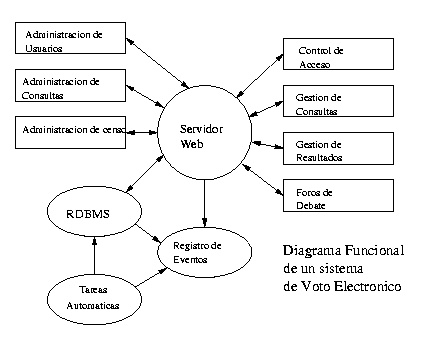
\includegraphics[width=10cm]{Figuras/funcdiag.jpg}
\caption{Diagrama funcional de un programa de voto}
Autor:  
\end{figure}

Básicamente, podemos descomponer el programa en diversas subestructuras:

\subsubsection*{Base de datos}
Cualquier sistema de voto deberá tener al menos las siguientes tablas de datos:

\begin{itemize}
\item Registro de datos personales
\item Registro de censo electoral
\item Registro de votaciones
\item Registro de resultados
\end{itemize}

Dichas tablas se organizan según un sistema de dependencias. La figura ilustra las dependencias entre tablas que utiliza Free-Vote

\begin{figure}[h!]
\centering
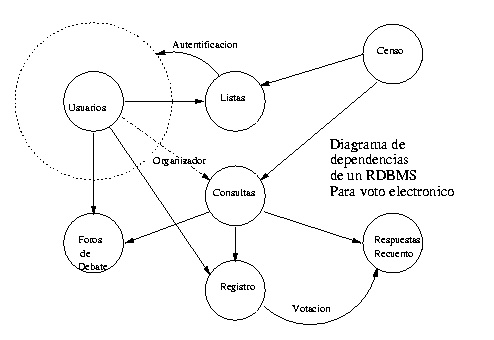
\includegraphics[width=10cm]{Figuras/rdbms.jpg}
\caption{Estructura de la base de datos}
Autor:  
\end{figure}

\subsubsection*{Gestión de usuarios}
Deberemos tener programas para realizar las siguientes tareas:
\begin{itemize}
\item Registro, alta, baja, y modificación de usuarios
\item Control de contraseñas, tarjeta de voto, etc
\item Seguimiento, seguridad, autentificación
\item Interacción con el correo electrónico
\end{itemize}

\subsubsection*{Gestión de consultas}
\begin{itemize}
\item Creación de consultas
\item Validación de usuarios y votos
\item Recuento de votos
\item Presentación de resultados
\item Persistencia de las votaciones dentro del sistema
\end{itemize}

\subsubsection*{Foros de debate. Chat y sistemas de comunicaciónes en línea}
Es muy común la existencia de foros de debate asociados a cada consulta. En ellos, los usuarios manifiestan las diversas opiniones sobre las consultas y sus resultados:

\begin{itemize}
\item Gestión del foro
\item Envío y recepción de mensajes
\end{itemize}

No sólo sistemas de foros son posibles. Algunos entornos incluyen sistemas de chat o de videoconferencia. Dependiendo del grado de interactividad que se pretenda, y de la complejidad del servidor, estos sistemas estarán o no presentes.

\subsubsection*{Correo electrónico}
Hemos tratado anteriormente, cómo el correo electrónico debería ser el medio principal de comunicación entre el servidor y el usuario. Lo utilizaremos para:

\begin{itemize}
\item Notificaciones
\item Envio de datos sensibles
\item En general todo tipo de información generada en el servidor, de interés para el usuario
\end{itemize}
Dependiendo del sistema, el grado de verbosidad será mayor o menor: Algunos sistemas envín información sobre consultas de manera automática; en otros es responsabilidad del organizador notificar a los interesados la existencia o incidencias relacionadas con alguna consulta.

\subsubsection*{Mecanismos de administración remota}
Dependiendo de la complejidad del sistema, las tareas de administración serán más o menos compleja. Lo normal es que el o los administradores tengan acceso directo al servidor, y puedan realizar directamente sobre el sistema las tareas de administración

En ocasiones esto puede ser o no conveniente, por lo que algunos sistemas incorporan mecanismos de administración remota. Esto permite además definir niveles de privilegios. Podemos identificar diversas tareas de administración:

\begin{itemize}
\item Altas y bajas
\item Modificaciones
\item Gestión de recursos
\item Gestión de incidencias
\end{itemize}

Por supuesto, al margen de estos sistemas, siempre existen los sistemas de gestión local, tanto automáticos como manuales.

Es necesario controlar estrictamente los recursos de administración: el responsable del sistema tiene acceso directo a las bases de datos y a su integridad y contenido. Al responsable del sistema se le asume integridad, pero nunca está de más una ayudita electrónica... chequeos, controles de integridad, registros automáticos de eventos, etc.


\subsubsection{Herramientas de software libre disponibles para programas de consulta}
\subsubsection*{Los clientes libres}
El recurso básico de un sistema libre de voto electónico es el Web: Recordemos que el principio de libertad, nos obliga a huír de soluciones que liguen a un determinado software o sistema operativo. Si bien en el servidor no es tanto problema, es una razón sine qua non en el cliente de voto. El uso del web y del lenguaje html es una garantía de portabilidad

Por el mismo motivo huiremos de soluciones web propietarias o no extendidas: plug-ins, javascript, applets java. No podemos olvidar que cualquiera, con independencia de su sistema y recursos debe poder participar En resumen, el cliente será cualquier navegador web que soporte HTML-3.2, sin extensiones

\subsubsection*{El lado del servidor}
Aunque en el lado del servidor se dispone de más libertad, vamos a evaluar las herramientas necesarias y su disponibilidad como software libre.


\begin{itemize}
\item En primer lugar está el servidor de bases de datos. Necesitaremos software que soporte integridad referencial, agrupamiento de transacciones, actualizaciones en cascada.... En el momento de escribir estas líneas sólo tenemos un RDBMS libre que cumpla estas condiciones: PostGreSQL-7.X, distribuído bajo licencia BSD
\item Necesitamos, por supuesto un servidor Web. En este caso no hay duda ninguna: Apache es nuestra elección. No solo por su carácter de software libre, sino por su seguridad y estabilidad: el 60\% de los servidores Web de InterNet están basados en él. Deberemos añadir soporte para SSL (Secure Socket Layer), y de scripts CGI.
\item Para unir el sistema Web con el servidor de bases de datos, escogeremos un lenguaje de programación de CGI's. Aquí la disponibilidad de software es mucho más variada: Perl, PHP, e incluso ejecutables compilados, bien nativos o bien servlets Java. No obstante, por su sencillez y posibilidades de acceso a bases de datos,  PHP es una de las mejores elecciones
\item Por debajo de todo este entorno necesitaremos un entorno de desarrollo libre y un sistema operativo libre... FreeBSD, o GNU/Linux son las elecciones del momento.
\end{itemize}


\section{Desarrollo}
\subsection{Propósito del Informe}
Derivado de la necesidades de \textbf{Duoc UC},  desde ahora el mandante,  su dolor se encuentra en el poder gestionar de forma oportuna los requerimientos de los estudiantes,  como también,  generar instancia de decisión  y voto,  por lo cual,  es menester desarrollar un prototipo simple, sencillo y de gran alcance. Vale mencionar que el mandante informa no poseer herramientas de este tipo,  como también ningún tipo de infraestructura.

Este informe tiene como fin primario,  documentar los distintos procesos del diseño de prototipos, utilizando las metodologías y \textit{frameworks} estudiados en clases, como a su vez, presentarse como respuesta al proyecto semestral de la asignatura de diseño de prototipos.



\newpage
\subsection{Desafío y escenario en que se aplica}
El ajdhasdasdhkajdaskjdhakda hgchfghgfhgfh
\newpage
\subsection{Descripción de la Solución propuesta}
\newpage
\subsection{Imágenes del prototipo Físico y de Mockups}
\newpage
\subsection{Perfil de Usuarios en el que se enfoca la solución}
\newpage
\subsection{Tipo de técnicas de levantamiento de información}
\newpage
\subsection{Mapas y esquemas desarrollados}
\newpage
\subsection{Usuarios entrevistados y fotografías del proceso}
\newpage
\subsection{Fotografías del Proceso de Testing}
\newpage
\subsection{Diseño de la Solución MVP}
\newpage
\subsection{Imágenes  del prototipo físico mejorado  y descripción de los Prototipos Tecnológicos diseñados }
\newpage
\subsection{Listado de menciones positivas y negativas de los usuarios sobre lo testeado}
\newpage
\subsection{Mejoras principales a considerar.}

\include{Conclusion}
\section{Bibliografia}
\section{Glosario}


\end{document}